\documentclass[12pt]{report}
\renewcommand\bibname{References}
\usepackage[a4paper, width=150mm,top=25mm,bottom=25mm]{geometry}
\usepackage{amsmath}
\usepackage{amsfonts}
\usepackage{graphicx}
\usepackage{hyperref}
\usepackage[cache=false, outputdir=aux]{minted}
\usepackage{listings}
\usepackage{fancyhdr}
\usepackage{caption}
\pagestyle{fancy}
\setlength{\headheight}{14.49998pt}
% \fancyhead{}
\fancyhead[L]{\small\leftmark}
\fancyhead[R]{\small\rightmark}
\graphicspath{attachments/}


\title{
{\textbf{Distributed memory parallelization of Lax-Wendroff method}}\\
{\large TIFR-CAM,}\\[-5pt]
{\large Bangalore, India.}\\[1cm]
{
\includegraphics{attachments/tifrlogo.png}}
}

\author{
    {\textbf{Report by:}}\\Devansh Tripathi\\{IVR No. IMS22090}\\{IISER Thiruvananthapuram,}\\{Kerala, India}\\[1 cm]
    {Period: June-July, 2024}
}
\date{}
\begin{document}
\maketitle
\chapter*{Acknowledgement}
I would like to ..

\chapter*{\centering\title{Distributed memory parallelization of Lax-Wendroff method}\\[1cm]}
\author{\centering
    {\textbf{Author}}\\Devansh Tripathi\\{IISER Thiruvananthapuram,}\\{Kerala, India}\\[4 cm]
    {\textbf{Supervisor}}\\{ Prof. Praveen Chandrashekar}\\{TIFR-CAM,}\\\hspace{171pt}{Bangalore, India}
}\\

\chapter*{Aim of the project}
The real world problems requires massive amount of data generation and needs compute power of more than a few computing units such as CPU/GPUs. The aim of this project is to tackle the issue of usage of \textbf{distributed memory on multiple nodes and to use the computing power of CPUs present on more than a node in an multi-node environment for an adaptive high-order numerical simulation framework for hyperbolic conservation laws --- \href{https://www.example.com}{\ttfamily TrixiLW.jl}} \vspace{15pt}

In order to extend {\ttfamily TrixiLW.jl} to support distributed memory parallelization --- Message Passing Interface (MPI) implementation is used. MPI is an open source implementation for parallelization developed and maintained by \href{https://www.mpi-forum.org/}{MPI Forum}. Optimization of MPI code have alse been performed in order to get good speed-up and higher efficiency as demonstrated by the results of scaling tests.


\tableofcontents

\chapter{Introduction}
% \section{Introduction}
Lax-Wendroff Flux Reconstruction (LWFR) is a high order, explicit spectral element method for solving systems of partial differential equations in cosservative form. 
\begin{equation}
    \boldsymbol{u}_t + \nabla_x \cdot \boldsymbol{f^a(u)} - \nabla_x \cdot \boldsymbol{f^v}(\boldsymbol{u},\nabla \boldsymbol{u}) = \boldsymbol{S(u)}
\end{equation}
An example of above system is the \href{https://en.wikipedia.org/wiki/Navier%E2%80%93Stokes_equations}{compressible Navier-Stokes equations.} Traditional spectral element methods for solving these equations are the Runge-Kutta Flux Reconstruction (RKFR) schemes which perform a spatial discretization (i.e., in x) and then use a \textbf{multi-stage} Runge-Kutta ODE solver to perform time discretization (i.e., in t). The Runge-Kutta method requires multiple inter-element communication for each of its stages which can become the bottleneck, especially in a parallel code.  

Lax-Wendroff Flux Reconstruction (LWFR) schemes are an alternative to this as they perform the evolution in a single stage, thus decreasing the inter-element communication. The main goal while writing parallel algorithm should be to minimize the data to be communicated without creating redundant data in each process's memory. 

Using parallel algorithms has its own advantages and disadvantages but the gain that we acquire is far more than the loss for data and compute intensive problems.
\section{Advantages of parallelization}
\begin{itemize}
    \item Execution of code on many nodes each with its own computing units enables to use extra compute.
    \item Execution of memory intensive programs on a multi-node environment enables it to use memeory available on each node.
    \item Using multiple cores on many nodes can speed up the process and can save time.
\end{itemize}

\section{Challenges of parallelization}
\begin{itemize}
    \item Execution of code in an multi-node environment requires a lot of resources such as computing units, interconnects, networking hardwares etc.
    \item Data communication between processes puts a additional overhead to the execution time which can be significant if code is not written efficiently.
    \item It increases the complexity of the code hence it is difficult to develop, modify and maintain the parallel code.
\end{itemize}
In chapter \ref{tf}, we will discuss the theoritical framework for LWFR method. I have also included finite volume method (FVM) as background for the LWFR as knowing about FVM can be very helpful to comprehend flux reconstruction method.

\vspace{5pt}\hspace{-26pt}
In chapter \ref{m}, I have explained the methodology of how parallelization of \linebreak {\ttfamily TrixiLW.jl} has been done. I also have mentioned about the data structures that has been used for parallelization.
Along with the methodology that we have followed, I have also provided a alternate way of parallelization using the newly released MPI Remote memory access (RMA) in chapter \ref{am}

\vspace{5pt}\hspace{-23pt}
In chapter \ref{ai}, I have performed analysis of results in terms of speed and accuracy, and provided a possible interpretation of results.

\vspace{5pt}\hspace{-23pt}
In later chapters \ref{c} and \ref{ra}, the conclusion and the results that we got from the code along with results of scaling tests are shown.

\begin{center}
    \rule{3cm}{1pt}
\end{center}


\chapter{Theoretical framework} \label{tf}
\section{Finite Difference Method} \label{fdm}
In this section the finite difference method for solving partial differential equations (PDEs) will be discussed. A finite difference method consists of the following steps:
\begin{enumerate}
    \item Discretization of the domain on which the equation is defined.
    \item For each grid point, replace the derivatives with an approximation, using the values in neighbouring grid points.
    \item Solve the resulting system of equations.
\end{enumerate}
There are set of approximations that are used to approximate the derivative. These includes-\\
For first derivative $f'$:
\begin{equation} \label{eqfdm}
f'(x)\approx 
\begin{cases}
    \frac{f(x+h) - f(x)}{h}, & \text{Forward difference }\\
    \frac{f(x) - f(x-h)}{h}, & \text{Backward difference} \\
    \frac{f(x+h) - f(x-h)}{2h}, & \text{Central difference.}
\end{cases}
\end{equation}
The commonly used approximation to second derivative $f''(x)$ is-
\begin{equation} \label{eqdouble}
    f''(x) \approx \frac{f(x+h) - 2f(x) + f(x-h)}{h^2}
\end{equation}
Now, we will see the approach to numerically solve a time-dependent PDE using finite difference methods.
\subsection{Semi-discretization}
This technique is used to discretize the time dependent PDEs. The word {\em semi} is to describe the notion that the PDE will first be discretize in space using finite difference methods and then some time marching schemes such as Runge-Kutta methods, Lax-Wendroff method etc., will be used to move forward in time. We will show this for a linear advection equation in 1D mesh
\begin{equation} \label{1}
    u_t + f(u)_x = 0
\end{equation}
In order to discretize the second derivaitve in above equation, we will use central differences-
\begin{equation} \label{eq 2}
    \frac{\partial u}{\partial t} = -\frac{f(x+h) - f(x-h)}{2h}
\end{equation}
The eq (\ref{eq 2}) is called semi-discretize form of the linear advection equation. In the next section, we will be using classical Lax-Wendroff method as our time marching scheme.
\subsection{Classical Lax-Wendroff method}
Lax-Wendroff schemes are used for numerically solving conservation law or a system of hyperbolic conservation laws. These methods belongs to the class of conservative schemes and can be derived in various ways. For simplicity, we will derive the method by using model given in equation (\ref{1}), namely the linear advection equation with $f(u)=au$, where $a$ is a constant propagation velocity. We can use Taylor expansion of $u_j^{n+1}$
\begin{equation*}
    u_j^{n+1} = u_j^n + \Delta t \frac{\partial u}{\partial t}\bigg\vert_j^n + \frac{(\Delta t)^2}{2} \frac{\partial^2 u}{\partial t^2}\bigg\vert_j^n + O(\Delta t^3)
\end{equation*}
It is a secong order accurate method since we are retaining terms till second order. From the equation (\ref{1}), we get by differentiation\\
\begin{minipage}{0.5\textwidth}
\begin{equation*}
    \frac{\partial u}{\partial t}\bigg \vert_j^n = -a\frac{\partial u}{\partial x}\bigg \vert_j^n \\
\end{equation*}
\end{minipage} \hspace{-40pt} and \hspace{-40pt}
\begin{minipage}{0.5\textwidth}
\begin{equation*}
    \frac{\partial^2 u}{\partial t^2}\bigg \vert_j^n = -a^2\frac{\partial^2 u}{\partial x^2}\bigg \vert_j^n 
\end{equation*}
\end{minipage}\\
We can use central difference from equation(\ref{eqfdm}) and from equation(\ref{eqdouble}) and the final result will be
\begin{align*}
    u_j^{n+1} &= u_j^n - a\Delta t \left(\frac{u_{j+1}^n - u_{j-1}^n}{2\Delta x}\right) - a\frac{(\Delta t)^2}{2} \left(\frac{u_{j+1}^n - 2u_j^n + u_{j-1}^n}{(\Delta x)^2}\right)\\ \\
    u_j^{n+1} &= u_j^n -\frac{a}{2}\frac{\Delta t}{\Delta x}\left(\frac{u_{j+1}^n - u_{j-1}^n}{2\Delta x}\right) - \frac{a}{2}\left(\frac{\Delta t}{\Delta x}\right)^2 \left(\frac{u_{j+1}^n - 2u_j^n + u_{j-1}^n}{(\Delta x)^2}\right)
\end{align*}
This is the update step for Lax-Wendroff. Later, we will see in section \ref{cfl}, how to calculate $\Delta t$ using CFL condition which is a needed but not a sufficient condition for stability of the scheme. The {\ttfamily Julia} implementation of this scheme is shown in the section \ref{i} of chapter \ref{am}.
\section{Finite Volume Methods}
\subsection{Motivation for Finite Volume Method}
In finite difference methods, the derivatives are approximated by finite differences -- esssentially using Taylor expansion. A large discussion on finite difference  methods shows that they need the solution to be smooth and equation to be satisfied point-wise. However, the solutions to the scalar conservation law (\ref{1}) are not necessarily smooth, so the Taylor expansion -- replacing derivatives using finite differences -- is no longer valid. Hence, we need a new framework for designing numerical methods for scalar conservation laws.

This section introduces the finite volume method for the numerical solution of hyperbolic PDE and system of hyperbolic PDEs. We will talk about fundamental concept of this method and also discuss a type of numerical flux. 

\subsection{Formulation for conservation laws}
The basic difference between finite difference methods and finite volume methods is that finite volume methods are derived on the basis of integral form of the conservation laws, instead of the differential form as in finite differences.

For the case of one spatial dimension as in eq (\ref{1}) the domain is divided into finite volumes (or \textit{grid cells/intervals}) and we need to monitor the approximation to the integral of $u$ over each of these volumes. For each time step, we need to update $u$ using the approximation to the flux $f(u)$ that comes in and goes out from the boundary of these volumes.

If we denote $i$ th volume by:
\begin{equation}
C_i = (x_{i-1/2},x_{i+1/2})
\end{equation}
The value $U^n_i$ will approximate the average value of $u$ over the $i$th interval at time $t^n$
\begin{equation}
U_i^n \approx \frac{1}{\Delta x}\int_{x_{i-1/2}}^{x_{i+1/2}} u(x, t_n) dx
\end{equation}
where $\Delta x=x_(i+1/2)-x_(i-1/2 )$ is the length of the cell. Here we are assuming a uniform grid for easeness of explanantion.\\
$\sum_{i=1}^N U_i^n \Delta x$ approximates the integral of $u$ over the entire $1D$ domain and if we use the method that is in conservative form, the value of $\sum_{i=1}^N U^n_i \Delta x$ will only change due to the fluxes at the boundary of the domain.\\
Now, we will see how can we develop an explicit time-marching algorithm using integral form of the conservation law. We can get integral form by integrating (\ref{1}) on interval $C_i$. Steps have been shown below:
\begin{gather*}
\int_{C_i}\frac{d}{dt} u(x,t_n) dx +\int_{C_i} \frac{d}{dx} f(u(x,t_n)) = 0 \\
\frac{d}{dt}\int_{C_i}u(x, t_n)dx =  f(u(x_{i-1/2}, t_n)) - f(u(x_{i+1/2},t_n))
\end{gather*}
For given $U_i^n$, the cell averages at time $t_n$, we can approximate the cell averages at time $t_{n+1}$, $U_i^{n+1}$, after a time step of length $\Delta t = t_{n+1} - t_n$. \\
Integrating the above equation in time from $t_n$ to $t_{n+1}$:
\begin{align*}
\int_{t_n}^{t_{n+1}} \frac{d}{dt} \int_{C_i} u(x, t_n) dx &= \int_{t_n}^{t_{n+1}} f(u(x_{i-1/2}, t_n)) - f(u(x_{i+1/2}, t_n)) \\
\int_{C_i} u(x, t_{n+1})dx - \int_{C_i} u(x, t_n)dx &=  \int_{t_n}^{t_{n+1}} f(u(x_{i-1/2}, t_n)) dt - \int_{t_n}^{t_{n+1}} f(u(x_{i+1/2}, t_n)) dt
\end{align*}
Rearranging this equation and dividing both sides by $\Delta x$ yields:
\begin{align} \label{4}
\begin{split}
\frac{1}{\Delta x} \int_{C_i} u(x, t_{n+1}) dx &= \frac{1}{\Delta x} \int_{C_i} u(x, t_n) dx \\ &- \frac{1}{\Delta x} \left[ \int_{t_n}^{t_{n+1}} f(u(x_{i-1/2}, t_n)) dt -  \int_{t_n}^{t_{n+1}} f(u(x_{i+1/2}, t_n)) dt \right]
\end{split}
\end{align}

In (\ref{4}), we can not evaluate the time integrals on the right hand side exactly, as $u(x_{i\pm1/2})$ varies with time along each edge of the cell. We can rewrite eq (\ref{4}) as:
\begin{equation}
U_i^{n+1} = U_i^n - \frac{\Delta t}{\Delta x} \left(F_{i+1/2}^n - F_{i-1/2}^n \right)
\end{equation}
where $F_{i-1/2}^n $ is the \textit{average} flux along $ x = x_{i-1/2}$:
\begin{equation*}
F_{i-1/2}^n  =  \frac{1}{\Delta t} \int_{t_n}^{t_{n+1}} f(u(x_{i-1/2},t_n)) dt
\end{equation*}
If we can approximate this \textit{average flux} function based on the values of $U^n$, then we will have a discrete method. And that approximation to \textit{average flux}  function is called \textit{numerical flux function}.

\subsection{The CFL Condition} \label{cfl}
The \textit{numerical flux} function as the approximation of \textit{average flux} is the main ingredient in a finite volume scheme. We need a approximation to:
\begin{equation}
\bar{F}^n_{j+1/2} \approx F^n_{i-1/2} =  \frac{1}{\Delta t}\int_{t_n}^{t^{n+1}} f(u(x_{i-1/2}, t_n)) dt
\end{equation}
at each interface $x_{i-1/2}$. As the cell averages $U^n_j$ are constant in each cell $C_j$, at each time level, we can define at each cell interface $x_{i-1/2}$ a, \textit{Riemann problem}:
\begin{equation} \label{7}
\begin{cases}
u_t + f(u)_x = 0 \\
u(x, t_n) = & \hspace{-28pt}
\begin{cases}
u^n_j  &  \text{if} \hspace{4pt} x < x_{j-1/2} \\
u^n_{j+1} & \text{if} \hspace{4pt} x > x_{j-1/2}
\end{cases}
\end{cases}
\end{equation}
At every time level, the cell averages define a superposition of $Riemann$ problems of the form (\ref{7}), at each interface. The solution to the $Riemann$ problem consists of shock waves, rarefraction and compound waves. Moreover, waves from neighboring \textit{Riemann} problems can intersect after some time hence imposing the CFL condition is a requirement. We define \textit{Courant number} as:
\begin{equation} \label{8}
v = \frac{\Delta t}{\Delta x} \max_p\mid\lambda^p\mid
\end{equation}
where $\lambda$'s are the $eigenvalues$ of a matrix $A$ in the case of system of linear hyperbolic equations and $\lambda$ can be the wave propogation speed in the case of a single hyperbolic PDE.

For a three point stencil the CFL condition leads to $v \leq 1$. It can be noted that for a wider stencils, the CFL condition can give $v \leq 2$. The CFL condition is a $necessary$ but not a sufficient condition for stability of the solution.
\subsection{Rusanov's flux}
Rusanov scheme \cite{rusanov} is also called {\em local Lax-Friedrich scheme} \cite{notes_ncm} because it can be obtained from a simple modification in {\em Lax-Friedrich scheme} basically using different approach in choosing the parameter $\lambda$. \vspace{8pt}
\hrule \vspace{8pt}
\hspace{-17pt}\textbf{A Note about Lax-Friedrich scheme}\\
Lax-Friedrich scheme has this structure:
\begin{equation}
    f_{j+1/2} = \frac{1}{2}\left(f_j + f_{j+1} \right) - \frac{1}{2}\lambda \left(u_{j+1} - u_j \right) \hspace{20pt} \lambda = \frac{\Delta x}{\Delta t}
\end{equation} 
The time step must satisfy the CFL condition \ref{cfl}, we can write time step $\Delta t$ as:
\begin{equation*}
    \Delta t = \text{CFL}\frac{\Delta x}{\max\limits_{j} \sigma(f'(u_j^n))}, \hspace{10pt} CFL \leq 1
\end{equation*}
where $\sigma$ is the {\em spectral radius}. We see that
\begin{equation*}
    \lambda \approx \max\limits_j \sigma(f'(u_j^n))
\end{equation*}
The parameter $\lambda$ is related to the maximum wave speed in the whole computational domain. The only problem with this scheme is this the results will be very {\em diffusive} and shocks are smeared to a considerable extent.
\vspace{5pt} \hrule \vspace{5pt}
In Rusanov's scheme, instead of global maximum we use local estimate of $\lambda$ and hence the flux has the form
\begin{equation}
    f_{j+1/2} = \frac{1}{2}(f_j + f_{j+1}) - \frac{1}{2} \lambda_{j+1/2}(u_{j+1} - u_j)
\end{equation}
where $\lambda_{j+1/2}$ is an estimate of the maximum wave speed arising in the Riemann problem at the face $j+1/2$. For Euler equations
\begin{equation*}
    \lambda_{j+1/2} = \max\{|u_j| + a_j, |u_{j+1}| + a_{j+1}\}
\end{equation*} is a good choice.

\section{Flux Reconstruction}
The flux reconstruction (FR) method is a class of discontinuous Spectral Element Method for the discretization of conservation laws. FR method utilizes a nodal basis which is usually based on some solution points like Gauss point etc., to approximate the solution with piecewise polynomials inside the element. The main idea is to constuct a continuous approximation of flux utilizing a numerical flux (discontinuous) at the cell interfaces and a {\em correction function}. The solution at the nodes is then updated by a collocation scheme in combination with a Runge-Kutta method.

The choice of the correction function affects the accuracy and stability of the method. FR method can be shown to be equivalent to some discontinuous Galerkin and spectral difference schemes, using a proper choice of solution points and correction function, as shown in \cite{trojak, hyunh}. The quadrature-free nature of FR method together with the ability to cast the operations as matrix-vector operations makes these methods to be performed efficiently on modern vector processors \cite{vincent}.

At some time $t$, we have the piecewise polynomial solution defined; the FR scheme can be explained by the following steps: \\ \\ 
Considering scalar form of conservation law $ u_t + f(u)_x = 0$ \\
\textbf{Step 1.} In each element, we contruct a flux approximation by interpolating the flux at the solution points leading to a polynomial of degree $N$, given by
\begin{equation*}
    f_h^\delta(\xi,t) = \sum_0^Nf(u_j^e(t))l_j(\xi)
\end{equation*}
where $\xi \in [0,1]$ is a point in reference element $[0,1]$
and $l_j$ is Lagrange polynomial of degree $N$. The above flux is discontinuous flux across the interfaces of the elements. \\ \\
\textbf{Step 2.} Continuous flux approximation is build by adding correction terms at the element boundaries
\begin{align*}
    f_h(\xi,t) = \left[ f_{e-\frac{1}{2}}(t)-f_h^\delta(0,t) \right]g_L(\xi)+ f_h^\delta(\xi,t) + \left[ f_{e+\frac{1}{2}}(t)-f_h^\delta(1,t) \right]g_R(\xi)
\end{align*}
where $g_L$, $g_R$ are correction functions at left and right boundary respectively, and 
\begin{equation*}
    f_{e+1/2} = f(u_h(x^-_{e+\frac{1}{2}},t),u_h(x^+_{e+\frac{1}{2}},t))
\end{equation*}
is a numerical flux that makes the flux unique across the cells.\\ \\
\textbf{Step 3.} \label{step3} Then we obtain the system of ODE by collocating the PDE at the solution points
\begin{equation*}
    \frac{du^e_j}{dt}(t) = -\frac{1}{\Delta x_e}\frac{\partial f_h}{\partial \xi}(\xi_j,t), \hspace{22pt} 0 \leq j \leq N
\end{equation*}
which can be solved in time by schemes such as Runge-Kutta.
\paragraph{Correction functions.} The correction functions $g_L$ and $g_R$ at the left and right boundary respectively, should satisfy few conditions in order to get a working scheme.\\
\textbf{1.} The end point conditions:
\begin{align*}
    \begin{split}
        g_L(0) = 1,&~~~~~g_R(0) = 0\\
        g_L(1) = 0,&~~~~~g_R(1) = 1
    \end{split}
\end{align*}
which insure the continuity of the flux at interfaces.\\
\textbf{2.} They should \textbf{approximate zero} in some sense. This means that they should not add or subtract anything in flux inside the element. 
% \begin{equation*}
%     \int\limits_{x_{e-1/2}}^{x_{e+1/2}}g_L(x) dx = 0
% \end{equation*}
Two correction functions Radau and g2 are of major interest as they cooresponds to commonly used DG formulations.

\section[LWFR]{Lax-Wendroff Flux Reconstruction}
Lax-wendroff method is a numerical method for solving system of hyperbolic conservation laws. This method can be derived using Taylor's expansion. We will also use the PDE to rewrite some of the time derivatives in the expansion as spatial derivaitves. Using Taylor's expansion in time around $t = t_n$, we can write the solution at next time level as
\begin{equation} \label{9}
    u^{n+1} = u^n + \sum\limits_{m=1}^{N+1} \frac{\Delta t^m}{m!}\partial_t^mu^n + O(\Delta t^{N+2})
\end{equation}
We are retaining terms up to $O(\Delta t^{N+1})$ so the overall accuracy, in both space and time, is of the order $N+1$. The expected spatial error is expected to be of $O(\Delta x^{N+1})$.
Using the PDE, $ \partial_t u = -\partial_x f$, we can re-write the time derivatives in terms of spatial derivatives
\begin{equation*}
    \partial_t^m u = -\partial_t^{m-1} \partial_xf = -(\partial_t^{m-1}f)_x, \hspace{8pt} m = 1,2 \dots
\end{equation*}
Now eq(\ref{9}) becomes

\begin{align*}
    u^{n+1} &= u^n - \sum\limits_{m=1}^{N+1} \frac{\Delta t^m}{m!}(\partial_t^{m-1}f)_x + O(\Delta t^{N+2})\\
    &= u^n - \Delta t\left[\sum\limits_{m=0}^N\frac{\Delta t^m}{(m+1)!}\partial_t^mf \right]_x + O(\Delta t^{N+2})
\end{align*}
\begin{align}
    \hspace{-43pt}= u^n - \Delta t\frac{\partial F}{\partial x}(u^n) + O(\Delta t^{N+2}) \label{11}
\end{align}
where
\begin{equation*}
    F(u) = \sum\limits_{m=0}^N \frac{\Delta t^m}{(m+1)!}\partial_t^mf(u)
\end{equation*}
is the approximation to the time average flux as it can be written as average of truncated Taylor's expansion of the flux $f$ in time. 

As the step described in the previous section, we will first reconstruct the time average flux $F$ inside each element by a continous polynomial $F_h(\xi)$ using discontinous flux and correction functions. Then truncating the eq(\ref{11}), the solution at the nodes is update by a collocation scheme as follows
\begin{equation}
    (u_j^e)^{n+1} = (u_j^e)^n - \frac{\Delta t}{\Delta x_e}\frac{dF_h}{d\xi}(\xi_j), \hspace{18pt} 0 \leq j \leq N
\end{equation}
Above is the single step Lax-Wendroff update scheme for any order of accuracy.

\begin{center}
    \rule{3cm}{1pt}
\end{center}

\chapter{Profile of Organisation}
\textbf{Name of Organisation:} Centre for Applicable Mathematics\\
\textbf{Affiliation:} Tata Institute of Fundamental Research, Mumbai\\
\textbf{Website:} \href{https://www.math.tifrbng.res.in/}{https://www.math.tifrbng.res.in/}
\paragraph{About:}The Centre for Applicable Mathematics (CAM) is a premier research centre for mathematics and is part of the Tata Institute of Fundamental Research. Research at CAM is focused on mathematical analysis, theoretical and computational analysis of PDEs and their applications, and probability theory, complex analysis and related areas. CAM runs graduate student programmes that lead to a PhD in mathematics. There are several opportunities to visit and work at CAM (postdoctoral fellowships, short term visiting positions, summer programmes, etc). Members of CAM are actively engaged in outreach activities as well — ranging from working with gifted high school students to training researchers in the latest advancements at the frontiers of their disciplines.\\ \\
\textbf{Mail Address:} Tata Institute of Fundamental Research, Centre For Applicable Mathematics, Post Bag No 6503, GKVK Post Office, Sharada Nagar, Chikkabommsandra, Bangalore 560065, Karnataka, India\\ \\
\textbf{Email:} math [at] math [dot] tifrbng [dot] res [dot] in

\chapter{Methodology} \label{m}
\documentclass[12pt]{article}
\usepackage{amsmath}
\usepackage{amsfonts}
%\usepackage{minted}
%\usepackage{hvpygmentex}

\begin{document}
\section{TrixiLW.jl}
This chapter introduces the a numerical simulation framework for hyperbolic conservation laws based on rixi.jl package written in  It supports $2D$ simulations on cartesian, curvilinear and structured meshes. mmmk
\end{document}

\chapter{Alternative Methodology} \label{am}
\section{Remote Memory Access: MPI 3.0}
In the reign of parallel computing, there exist two major approaches for communicating data between processes:
message passing and direct memory access of the remote process. Shared memory approach is also there but that 
is limited to the procesess on the same node. 

MPI-1 provides a way for message passing between processes while MPI-2 gives approach for direct memory access of remote processes and MPI-3 extends it to a great extent. MPI RMA \cite{rmabook} uses operations like \textit{put}, \textit{get} and \textit{accumulate} to \textit{write}, \textit{read} and \textit{reduce} data respectively to a remote process without involving the remote process. One limitation of RMA approach is this it require special hardware support but with increasingly high development in networking caters this need to much extent.

\subsection{Shared memory vs RMA}
MPI remote memory access must be distinguished from shared memory programming model in the following ways:
\begin{itemize}
    \item MPI RMA approach can be used for communication between cores on the same node as well as cores on different
    nodes. While shared memory approach is limited to processes on the same core using \textit{threads}.
    \item In MPI RMA data can be accesses using {\ttfamily MPI\_Put} and {\ttfamily MPI\_Get} operations while in shared memory we can access data using usual load and store operations as shown in the pictures.
    \item In shared memory, we have a single address space, shared by multiple threads of execution while in RMA, programmer
    decides how much memory will be exposed to the remote process for communication. 
\end{itemize}
\begin{figure}
    \centering
    \begin{minipage}{.5\textwidth}
        \centering
        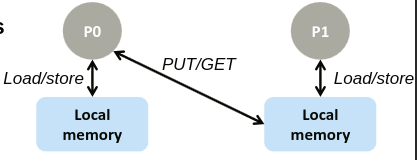
\includegraphics[width=0.78\linewidth]{attachments/rma.png}
        \caption{RMA$^1$}
    \end{minipage}%
    \begin{minipage}{.5\textwidth}
        \centering
        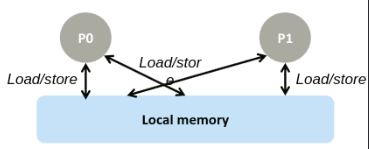
\includegraphics[width=0.78\linewidth]{attachments/shared_mem.png}
        \caption{Shared Memory$^1$}
    \end{minipage}
\end{figure}
The major disadvantage of shared memory model is \textit{simultaneous access by different threads to a same memory location.}
In order to avoid this race condition, many sophisticated techniques in compilers and special routines are needed such as 
\textit{locks and mutexes.}

\section{Introduction to RMA}
In traditional message passing, one process \textit{sends} data to other process using {\ttfamily MPI\_Send} and other 
process \textit{receives} data using {\ttfamily MPI\_Recv}. Every \textit{send} is compulsory to have a \textit{receive}
at the receiver process. This cooperative nature of MPI can impose order or need \textit{tag} matching for delivery of data
and that will have performance costs due to overheads.

MPI RMA provides a way of data communication from \textit{origin process} (process that sends data) to the \textit{target
process} (process to which data has been sent), without the involvement of \textit{target process}. The calling process specifies
both send and receive buffer. Since a single process is involved, these routines are also called \textit{one-sided routines}:

There are three main steps in using RMA:
\begin{itemize}
    \item \textbf{Defining a memory window:}\\
    Memory \textit{window} is collection of memory locations defined by a group of processes and only those locations can be
    modified by the remote process using RMA operations. This involves creation of a new MPI object {\ttfamily MPI\_Win}. There
    are $4$ window creation routines specified by MPI Forum.
    \item \textbf{Moving the data from \textit{origin} to \textit{target} process:}\\
    There are several routines to move the data between processes without the involve of the process instead directly writing the
    data into remote processes memory. These routines include: {\ttfamily MPI\_Put, MPI\_Get, MPI\_Accumulate} etc.
    \item \textbf{Specifying how do we know that data is available to remote process:}\\
    This is to say that how do we know that receive has been completed? There are several routines such as {\ttfamily MPI\_Win\_fence,
    MPI\_Win\_lock/unlock} etc. that makes sure that data is available to the target process for its local load/store operations.     
\end{itemize}

\subsection{Memory Window}
\begin{figure}[!ht]
    \centering
    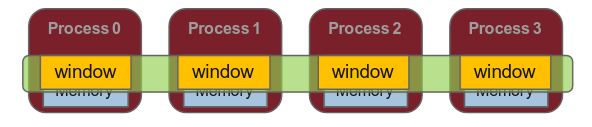
\includegraphics[width=0.75\linewidth]{attachments/mem_window.png}
    \caption{Memory window in RMA$^1$}
\end{figure}
It is the memory region of a process that can be accessed by another process using RMA operations. All or a group of processes can 
create a window or many windows by contributing some part of their memory to the window. It is a contiguous section of memory. There
are these $4$ window creation routines:
\begin{itemize}
    \item {\ttfamily MPI\_Win\_allocate:} In this routine memory allocation and window creation both are handled by MPI implemention.
    \item {\ttfamily MPI\_Win\_create:} This routine creates the window from already allocate memory. User have to provide some allocated
    memory to be create as a window.
    \item {\ttfamily MPI\_Win\_allocate\_shared:} This routine helps in creating a shared memory window from already allocate memory for
    the process on the same node hence these process can access each other data with simple load/store and avoid communication completely.
    \item {\ttfamily MPI\_Win\_create\_dynamic:} It creates a window but does not attach memory directly to it. Memory can be attached later
    using {\ttfamily MPI\_Win\_attach} and can be deattached using {\ttfamily MPI\_Win\_deattach}. 
\end{itemize}

By default, the memory that has been allocated by MPI implemention (if user specifies so) is {ttfamily contiguous} unless the
the {\ttfamily non-contiguous} option is {\ttfamily true.} This can have performance implications as well since {\ttfamily non-contiguous}
memory can be allocated aligning to the cache sizes which will decrease the number of cache misses.

After all the communication has been done and window is no longer required, it can be free using {\ttfamily MPI\_Win\_free} by all the 
processes that have created the window.\\
\hrule
\begin{listing}[!ht]
\begin{minted}[linenos]{Julia}
int MPI_Win_create(void *base, MPI_Aint size, int disp_unit,
                   MPI_nfo info, MPI_Comm comm, MPI_Win *win)
int MPI_Win_free(MPI_Win *win)
\end{minted}
\caption{Syntax for C}
\end{listing}
\hrule
\vspace{10pt}
There are few interesting parameters that are required by window calling routines:
\begin{itemize}
    \item \textbf{disp\_unit:} This argument unit should be the multiple of {\ttfamily sizeof()} of simple type such as `int` etc.
    that creates up the window object. For example if an array of {\ttfamily Floats} is making up the window then {\ttfamily disp\_unit}
    should be multiple of {\ttfamily sizeof(Float)}. This is the local unit size for displacements, in bytes.
    \item \textbf{info:} This arguemnt of only used for optimization purposes. A value {\ttfamily MPI\_INFO\_NULL} is always valid.
\end{itemize}

\subsection{Moving Data}
Since we have now seen how to make memory as a window for RMA opertaions, we need to specify how to move data between process.
MPI provides several routines to specify what data to move and to which location. Three of the simplest routines have been
described below:
\subsubsection{{\ttfamily \large MPI\_Put}}
\begin{figure}[!ht]
    \centering
    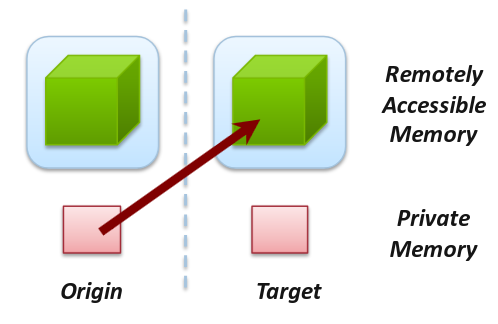
\includegraphics[width=0.35\linewidth]{attachments/put_rma.png}
    \caption{MPI\_Put$^1$}
\end{figure}
{\ttfamily MPI\_Put} is like a "store/write to remote memory" operation. It is a non-blocking communicating routine. This routines 
writes data from {\ttfamily origin} process's memory called {\ttfamily origin address} to {\ttfamily remote} process's memory at
the location as described by {\ttfamily displacement} argument. The data that need to be moved can be anywhere in the {\ttfamily origin}
process's memory, it need not to be inside a window.

Programmer need to pay attention while providing the {\ttfamily displacement} argument. \textbf{The destination of data is always relative
to the memory window exclusive to {\ttfamily remote} process not with the whole window object}.

MPI RMA operations define a separation between moving of data and completion of the operations. Window ~synchronization ~routines ~such as
{\ttfamily MPI\_Win\_fence} should be used after RMA opertions for completion of these operations. Between two {\ttfamily MPI\_Win\_fence} calls
any number of {\ttfamily MPI\_Put} operations can be issued. But if a {\ttfamily MPI\_Put} and {\ttfamily MPI\_Accumulate} operation overlaps (issued 
to same memory location) between two {\ttfamily MPI\_Win\_fence} calls then result will be {\ttfamily undefined behaviour.} Along with that,
{\ttfamily MPI\_Put} and {\ttfamily MPI\_Get} both can not be used within two {\ttfamily MPI\_Win\_fence} calls.

{\ttfamily MPI\_Put} is \textbf{not} an atomic operation. An \textbf{atomic operation} is an operation that can be completed within one CPU cycle and
hence these operation can not be interrupted in between by any other process. They execute at lowest level and cannot be broken further.
\begin{listing}[!ht]
\hrule \vspace{5pt}
\begin{minted}[linenos]{Julia}
int MPI_Put(const void *origin_addr,
            int origin_count, MPI_Datatype origin_datatype, int
            target_rank, MPI_Aint target_disp, int target_count,
            MPI_Datatype target_datatype, MPI_Win win)
\end{minted}
\caption{Syntax for C}
\hrule
\end{listing}

\subsubsection{{\ttfamily \large MPI\_Get}}
\begin{figure}[!ht]
    \centering
    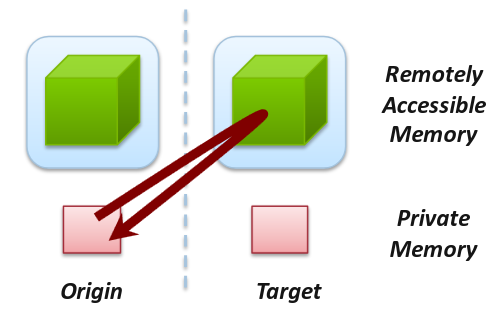
\includegraphics[width=0.35\linewidth]{attachments/get_rma.png}
    \caption{MPI\_Get$^1$}
\end{figure}
{\ttfamily MPI\_Get} routine is used to get data from remote process to the calling process. It can get data from remote process's window to anywhere 
in the origin (calling) process memory means {\ttfamily origin\_addr} need not to be inside window for calling process. This operation is also not an
\textbf{atomic} operation.\\
While calling this routine, programmer needs to specify the {\ttfamily displacement} argument relative to the window exclusive to the remote process.

This displacement arguement will specify the location of the data at remote process that needs to be written at the origin process's memory. After
using this routine, there should be a call to a window synchronization routine to ensure that the data has been received at the origin process.
\begin{listing}[!ht]
\hrule \vspace{5pt}
\begin{minted}[linenos]{Julia}
int MPI_Get(void *origin_addr, int origin_count, 
            MPI_Datatype origin_datatype, int target_rank,
            MPI_Aint target_disp, int target_count,
            MPI_Datatype target_datatype, MPI_Win win)
\end{minted}
\hrule
\caption{Syntax for C}
\end{listing}

\subsubsection{{\ttfamily \large MPI\_Accumulate}}
\begin{figure}[!ht]
    \centering
    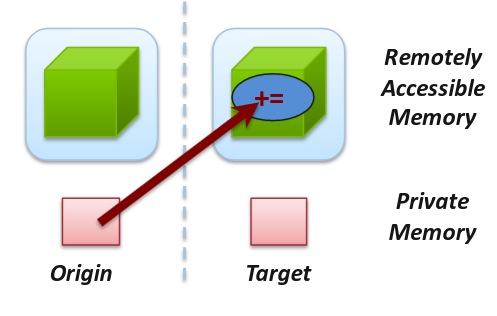
\includegraphics[width=0.35\linewidth]{attachments/accum_rma.png}
    \caption{MPI\_Accumulate$^1$}
\end{figure}
{\ttfamily MPI\_Accumulate} routine provides a way to move and combine data at the target process using any of the reduction operations such as
{\ttfamily MPI\_SUM, MPI\_MAX} etc. It can be seen similar to {\ttfamily MPI\_Reduce} operation but without the involvement of target process. There
are few restrictions for using {\ttfamily MPI\_Accumulate} as listed below:
\begin{itemize}
    \item It allows \textbf{only predefined operations} such as {\ttfamily MPI\_SUM, MPI\_MAX, MPI\_MIN, MPI\_LAND, MPI\_LOR} etc.
    \item It allows only \textbf{predefined} MPI datatypes and MPI derived datatypes where all components are of same predefined datatype.
\end{itemize}
\subsubsection{{\ttfamily MPI\_Accumulate as MPI\_Put}}
Since {\ttfamily MPI\_Accumulate} is an atomic operation while {\ttfamily MPI\_Put} is not an atomic operation and if we want to use atomic
{\ttfamily  MPI\_Put} we can achieve this using {\ttfamily MPI\_Replace} as an operation of {\ttfamily MPI\_Accumulate}. This will put the value in {\ttfamily origin\_addr} buffer to the target location as provided while calling this routine.

\begin{listing}[!ht]
\hrule \vspace{5pt}
    \begin{minted}[linenos]{Julia}
int MPI_Accumulate(const void *origin_addr, int origin_count,
                MPI_Datatype origin_datatype, int target_rank,
                MPI_Aint target_disp, int target_count,
                MPI_Datatype target_datatype, MPI_Op op,
                MPI_Win win)
    \end{minted}
\hrule
    \caption{Syntax for C}
\end{listing}

\subsection{Synchronization Routines}
Synchronization routines are a way to tell the process that data is available for local load/store operations from RMA operations as well as data is available for RMA operations from local load/store operations. They need to be called before as well as after RMA operations. The reason for calling them before RMA operations is to make sure that any local load/store operation that had been performed on the window object has been successfully completed and that data can be used in RMA operations. This can be omitted if there are no local load/store operations on the window before RMA operations. Later calling them will make sure the completion of RMA opertions itself.

There are two types of target synchronization in MPI RMA:
\begin{enumerate}
    \item Active Target synchronization.
    \item Passive Target synchronization.
\end{enumerate}

\subsubsection{\large Active Target synchronization} 
Active target synchronization involves both the origin and the target processes in synchronization using {\ttfamily MPI\_Win\_fence}. Any MPI RMA calls need to be wrapped by {\ttfamily MPI\_Win\_fence} call.

\subsubsection{\textbf{MPI\_Win\_fence}}
{\ttfamily MPI\_Win\_fence} is a collective call to all processes in the group associated with the window object that has been passed to {\ttfamily MPI\_Win\_fence}. It makes sure that any local stores to the memory window will be visible to RMA operations before any RMA operation takes place. In any pair of successive {\ttfamily MPI\_Win\_fence} there may either be any local stores to the local memory window or {\ttfamily  MPI\_Put/Accumulate} calls but not both.If there no {\ttfamily MPI\_Put} operation in between two {\ttfamily MPI\_Win\_fence} call then there may be both load and {\ttfamily MPI\_Get} operations on the memory window. 

{\ttfamily assert} argument can be used to indicate exactly what kind of operation \linebreak{\ttfamily MPI\_Win\_fence} is synchronizing. Typically, it is used to separate {\ttfamily MPI\_Put/Accumulate} operations from local load and store operation. \vspace{10pt}
\hrule \vspace{-8pt}
\begin{minted}[linenos]{Julia}
int MPI_Win_fence(int assert, MPI_Win win)        
\end{minted}
\vspace{-8pt}
\hrule

\subsubsection{\large Passive Target synchronization}
In this synchronization, the target process does not need to call any synchronization routines such as {\ttfamily MPI\_Win\_fence}. Before starting any RMA call, there should be a {\ttfamily MPI\_Win\_lock} and after those calls there should be a {\ttfamily MPI\_Win\_unlock} but only on the origin proce. This means that all the RMA calls will get completed after {\ttfamily MPI\_Win\_unlock} returns.

{\ttfamily MPI\_Win\_unlock} ensures that the RMA operations have been completed successfully and all the data transfers are visible to the target memory esssentially all the synchronization is done by {\ttfamily MPI\_Win\_unlock}. There is another version of lock that locks the window on all the processes called {\ttfamily MPI\_Win\_lock\_all}. {\ttfamily MPI\_Win\_unlock\_all} is used to unlock the window then. But there is some restrictions on type of lock used for {\ttfamily MPI\_Win\_lock\_all}, it can only provide shared access using {\ttfamily MPI\_LOCK\_SHARED} and the exclusive.

{\ttfamily MPI\_Win\_lock} call is in itself a {\em non-blocking} call hence it will return the control to the calling process just after the call and it will not wait for the target process to {\em acquire} the lock except in the case when the target process is same as the calling process, there MPI standard specifies it to be a {\em blocking} call. 

Since {\ttfamily MPI\_Win\_unlock} performs the synchronization and that will be called at the end. But what if we want to use the communicated data before calling {\ttfamily  MPI\_Win\_unlock}? In that case, there are few routines available for synchronization before calling {\ttfamily MPI\_Win\_unlock}.\\
For Separate Memory Model: \footnote[2]{For memory models, see section \ref{model}}
\begin{itemize}
	\item {\ttfamily MPI\_Win\_flush}: This routine can do force completion of all RMA routines that has been called till that point, both at the `origin` as well as on target process.
	\item {\ttfamily MPI\_Win\_flush\_local}: This routine can complete all RMA operations locally for the process which is calling the RMA operations.
\end{itemize}
Hence, the buffers involved in pending RMA operations at the origin process can be re-used safely after calling above routine.\\
For Unified Memory Model: \footnotemark[2]
\begin{itemize}
	\item {\ttfamily MPI\_Win\_sync}: It synchronizes private memory with public memory window in passive RMA.
\end{itemize}
Unified model is indeed coherent but the timings of when the updates of public memory become visible in private memory is not explicitly defined hence it is advisable to use this function. \vspace{10pt}
\hrule \vspace{5pt} \hspace{-21pt}
\textbf{Note:}\\
Writing RMA program by having a memory model in mind may limits portability hence prefer {\ttfamily MPI\_Win\_flush} operation as they are available on both models. \vspace{5pt}
\hrule

\subsection{Memory models} \label{model}
\textbf{Separate memory model}\\
The entire RMA implementation is based on the concept of public and private memory. Local load and store operations use private memory while the RMA operations uses public (exposed) memory. In separate memory model, the private and public memory remains logically separated and public memory window holds copy of the variable from private memory. These type of model is generally used on \textbf{non-coherent} systems.

{\ttfamily MPI\_Win\_fence} essentially makes the sure that whatever changes were made to public memory has been copied to private memory as vice-versa. Different values of assert parameter can be provided to avoid unnecessary copying.The above reasoning also says that only RMA routines must be used to update memory location in window object.
\begin{figure}[!ht]
    \centering
    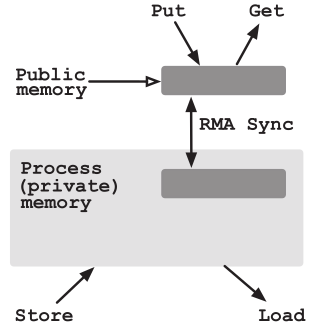
\includegraphics[width=0.35\linewidth]{attachments/sep_mem_model.png}
    \caption{Separate Memory Model$^1$}
\end{figure}\\
\vspace{3pt} \hspace{-11pt}
\textbf{Unified memory model}\\
In coherent systems, MPI implementations does not differentiate between the public and private memory i.e. changes made to private memory location will eventually become visible to public memory but the keyword here is {\em eventually}.

Hence programmers are advised to make sure the visibility of changes by using synchronization routines such as {\ttfamily MPI\_Win\_fence}, {\ttfamily MPI\_Win\_unlock} or {\ttfamily MPI\_Win\_Sync}
\begin{figure}[!ht]
    \centering
    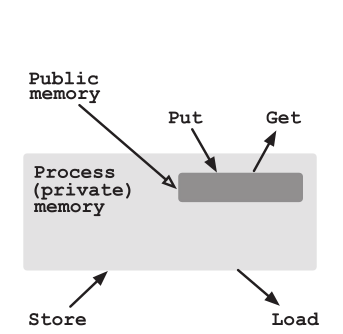
\includegraphics[width=0.37\linewidth]{attachments/uni_mem_model.png}
    \caption{Unified Memory Model$^1$}
\end{figure}
\hrule \vspace{5pt} \hspace{-21pt}
\textbf{Note:}\footnotetext[1]{All images credits: \cite{rma}}\\
To determine whether the MPI environment provides the unified or separate memory model, one can check the the MPI\_WIN\_MODEL attribute on the window. The value of this attribute is a pointer to an integer that can have one of two values: MPI\_WIN\_UNIFIED or MPI\_WIN\_SEPARATE for the unified and separate memory models, respectively.

\section{Implementation} \label{i}
In this section, we will discuss about the implementation of classical Lax-Wendroff method for linear advection equation using finite difference approach in 1D case. The theory related to finite difference approach can be found in section \ref{fdm} of chapter \ref{tf}. This is the parallel code implemented using MPI RMA.
\begin{minted}[linenos]{Julia}
# getting boundary values and halo exchanges
function get_ghost_values!(param, u, win)
    if size == 1
        u[1] = u[param.N_local]
        u[param.N_local + 2] = u[3]
        return
    end
    next = (rank + 1) % size
    if rank !== size - 1  
        buf1 = fill(0.0, 1)
        MPI.Win_lock(win; rank=next, type=MPI.LOCK_SHARED, nocheck=true)
        MPI.Put!(u[param.N_local+1], win; rank=next, disp=0)
        MPI.Get!(buf1, win; rank=next, disp=1)
        MPI.Win_unlock(win, rank=next)
        u[N_local+2] = buf1[1]
    else
        buf2 = fill(0.0, 1)
        MPI.Win_lock(win; rank=next, type=MPI.LOCK_SHARED, nocheck=true)
        MPI.Put!(u[param.N_local], win; rank=next, disp=0)
        MPI.Get!(buf2, win; rank=next, disp=2)
        MPI.Win_unlock(win; rank=next)
        u[N_local+2] = buf2[1]
    end
    MPI.Win_fence(win)
end
\end{minted}
The above code is writtten for periodic boundary conditions. {\ttfamily get\_ghost\_values!} function is the only function that required MPI communication and rest all code is serial. In above function, the first {\ttfamily if} block is to handle the case if total number of processes is 1 essentially the serial case. Now, talking about the main part related to MPI RMA, we are using {\ttfamily lock/unlock} mechanism hence this is passive target synchronization.

{\ttfamily MPI\_Put} has been used to write the values from {\ttfamily u[param.N\_local+1]} to the {\ttfamily next} rank at the displacement 0 means at the starting of the window of {\ttfamily next} rank. Then {\ttfamily MPI\_Get} has been used to get the values from {\ttfamily next} rank's displacement 1 to the buffer {\ttfamily buf1}. The displacement 1 simply means that we need to skip the first memory location in the window of the {\ttfamily next} rank. 

At the end, {\ttfamily MPI\_Win\_fence} is used in order to complete the store operations that we are performing at the location {\ttfamily u[N\_local+2]}. We can also omit the use of {\ttfamily MPI\_Get} completely and can just use {\ttfamily MPI\_Put}. By doing this, we also not need to perform the store operation at the last hence no need to use {\ttfamily MPI\_Win\_fence}. {\ttfamily nocheck=true} is an optimization option that will skip the check for access to the window by other processes as we know that the code is written in such a way that there won't be any illegal access attempts to the window. The optimization in MPI RMA is the responsibility of the programmer by providing such options. This is not the most optimized code and it can further be optimized. 

The reader should not get confused with {\ttfamily if} conditions as they are required due to periodic boundary conditions and subject to change as depends on boundary condition used.

In this project, I have also implemented the serial and parallel (MPI RMA) implementation of linear advection equation in 1D and 2D cases and is available on Github on this \href{https://github.com/Devansh1106/Sample-MPI-Julia/tree/main/linadv}{link.} 
\begin{center}
    \rule{3cm}{1pt}
\end{center}

\chapter{Analysis and Interpretation}\label{ai}
\section{Analysis of results}
In this project, multi-node parallelization of the existing serial code for simulation of conservation laws have been performed. Multi-node parallelization enables the program to use the capabilities of a server consists of several nodes and each node having various computing units connected with fast interconnects such as {\ttfamily InfiniBand}. Each node also have its own memory hence in order to get access to other process's memory we need to exclusively communicate the information that we want the other process to have access and there comes {\ttfamily MPI} into the picture.

The parallel code has been tested by running two problems: \textbf{Kelvin-Helmholtz instability} and \textbf{isentropic Euler vortex}. The scaling tests for both of these problems have been performed and results are shown.
\subsection{Speedup calculation}
The speed up results have been shown for the parallel code. These speedup results are in comparison to serial code execution time which is essentially running the parallel code with total number of process as 1. Formula used for calculation speedup is
\begin{equation*}
    \text{Speedup} = \frac{\text{Execution time with 1 process}}{\text{Execution time with N processes}}
\end{equation*}
For \textbf{Kelvin-Helmholtz instability}, \\
Execution time with 1 process: 68230.47 seconds\footnote[3]{All the data has been collected on Dual Intel(R) Xeon(R) Gold 6148 CPU @ 2.40GHz}\\
Execution time with 16 process: 5157.72 seconds
\begin{equation*}
    \text{Speedup} = \frac{68230.47}{5157.72} = 13.23~~\text{times}
\end{equation*}
\linebreak
For \textbf{isentropic Euler vortex},\\
Execution time with 1 processes: \footnotemark[3] \\
Execution time with 16 processes: 14904 seconds
\begin{equation*}
    \text{Speedup} = \frac{}{14904} = ~~\text{times}
\end{equation*}
\vspace{10pt}
\subsection{Efficiency calculation}
The efficiency of a parallel code is a measure of how effectively a parallel program is able to utilize the available computational resources compared to its sequential counterpart. It is calculated by:
\begin{equation*}
    \text{Efficiency} = \frac{\text{Speedup}}{\text{Number of processors}} \times 100 \%
\end{equation*}
For \textbf{Kelvin-Helmholtz instability},\\
Speedup = 13.23\\
Total number of processes = 16
\begin{equation*}
    \text{Efficiency} = \frac{13.23}{16} \times 100 \% = 82.7 \%   
\end{equation*}
\begin{figure*}[!ht]
    \centering
    \begin{minipage}{0.5\textwidth}
        \centering
        
\includegraphics[width=0.9\linewidth]{attachments/kelvin_8.0000.png}
        \caption*{(a)}
    \end{minipage}%
    \begin{minipage}{0.5\textwidth}
        \centering
        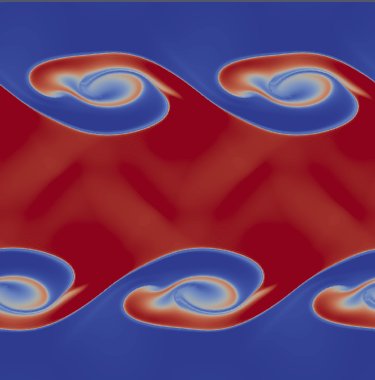
\includegraphics[width=0.9\linewidth]{attachments/kelvin_8.0264.png}
        \caption*{(b)}
    \end{minipage}
    \caption{Kelvin-Helmholtz instability at $t = 3$ using polynomial degree $N = 4$, (a) Initial condition, (b) density plot}
\end{figure*}

\hspace{-18pt}For \textbf{isentropic Euler vortex},\\
Speedup = \\
Total number of processes = 16
\begin{equation*}
    \text{Efficiency} = \frac{}{16} \times 100 \% =  \%   
\end{equation*}
\begin{figure*}[!ht]
    \centering
    \begin{minipage}{0.5\textwidth}
        \centering
        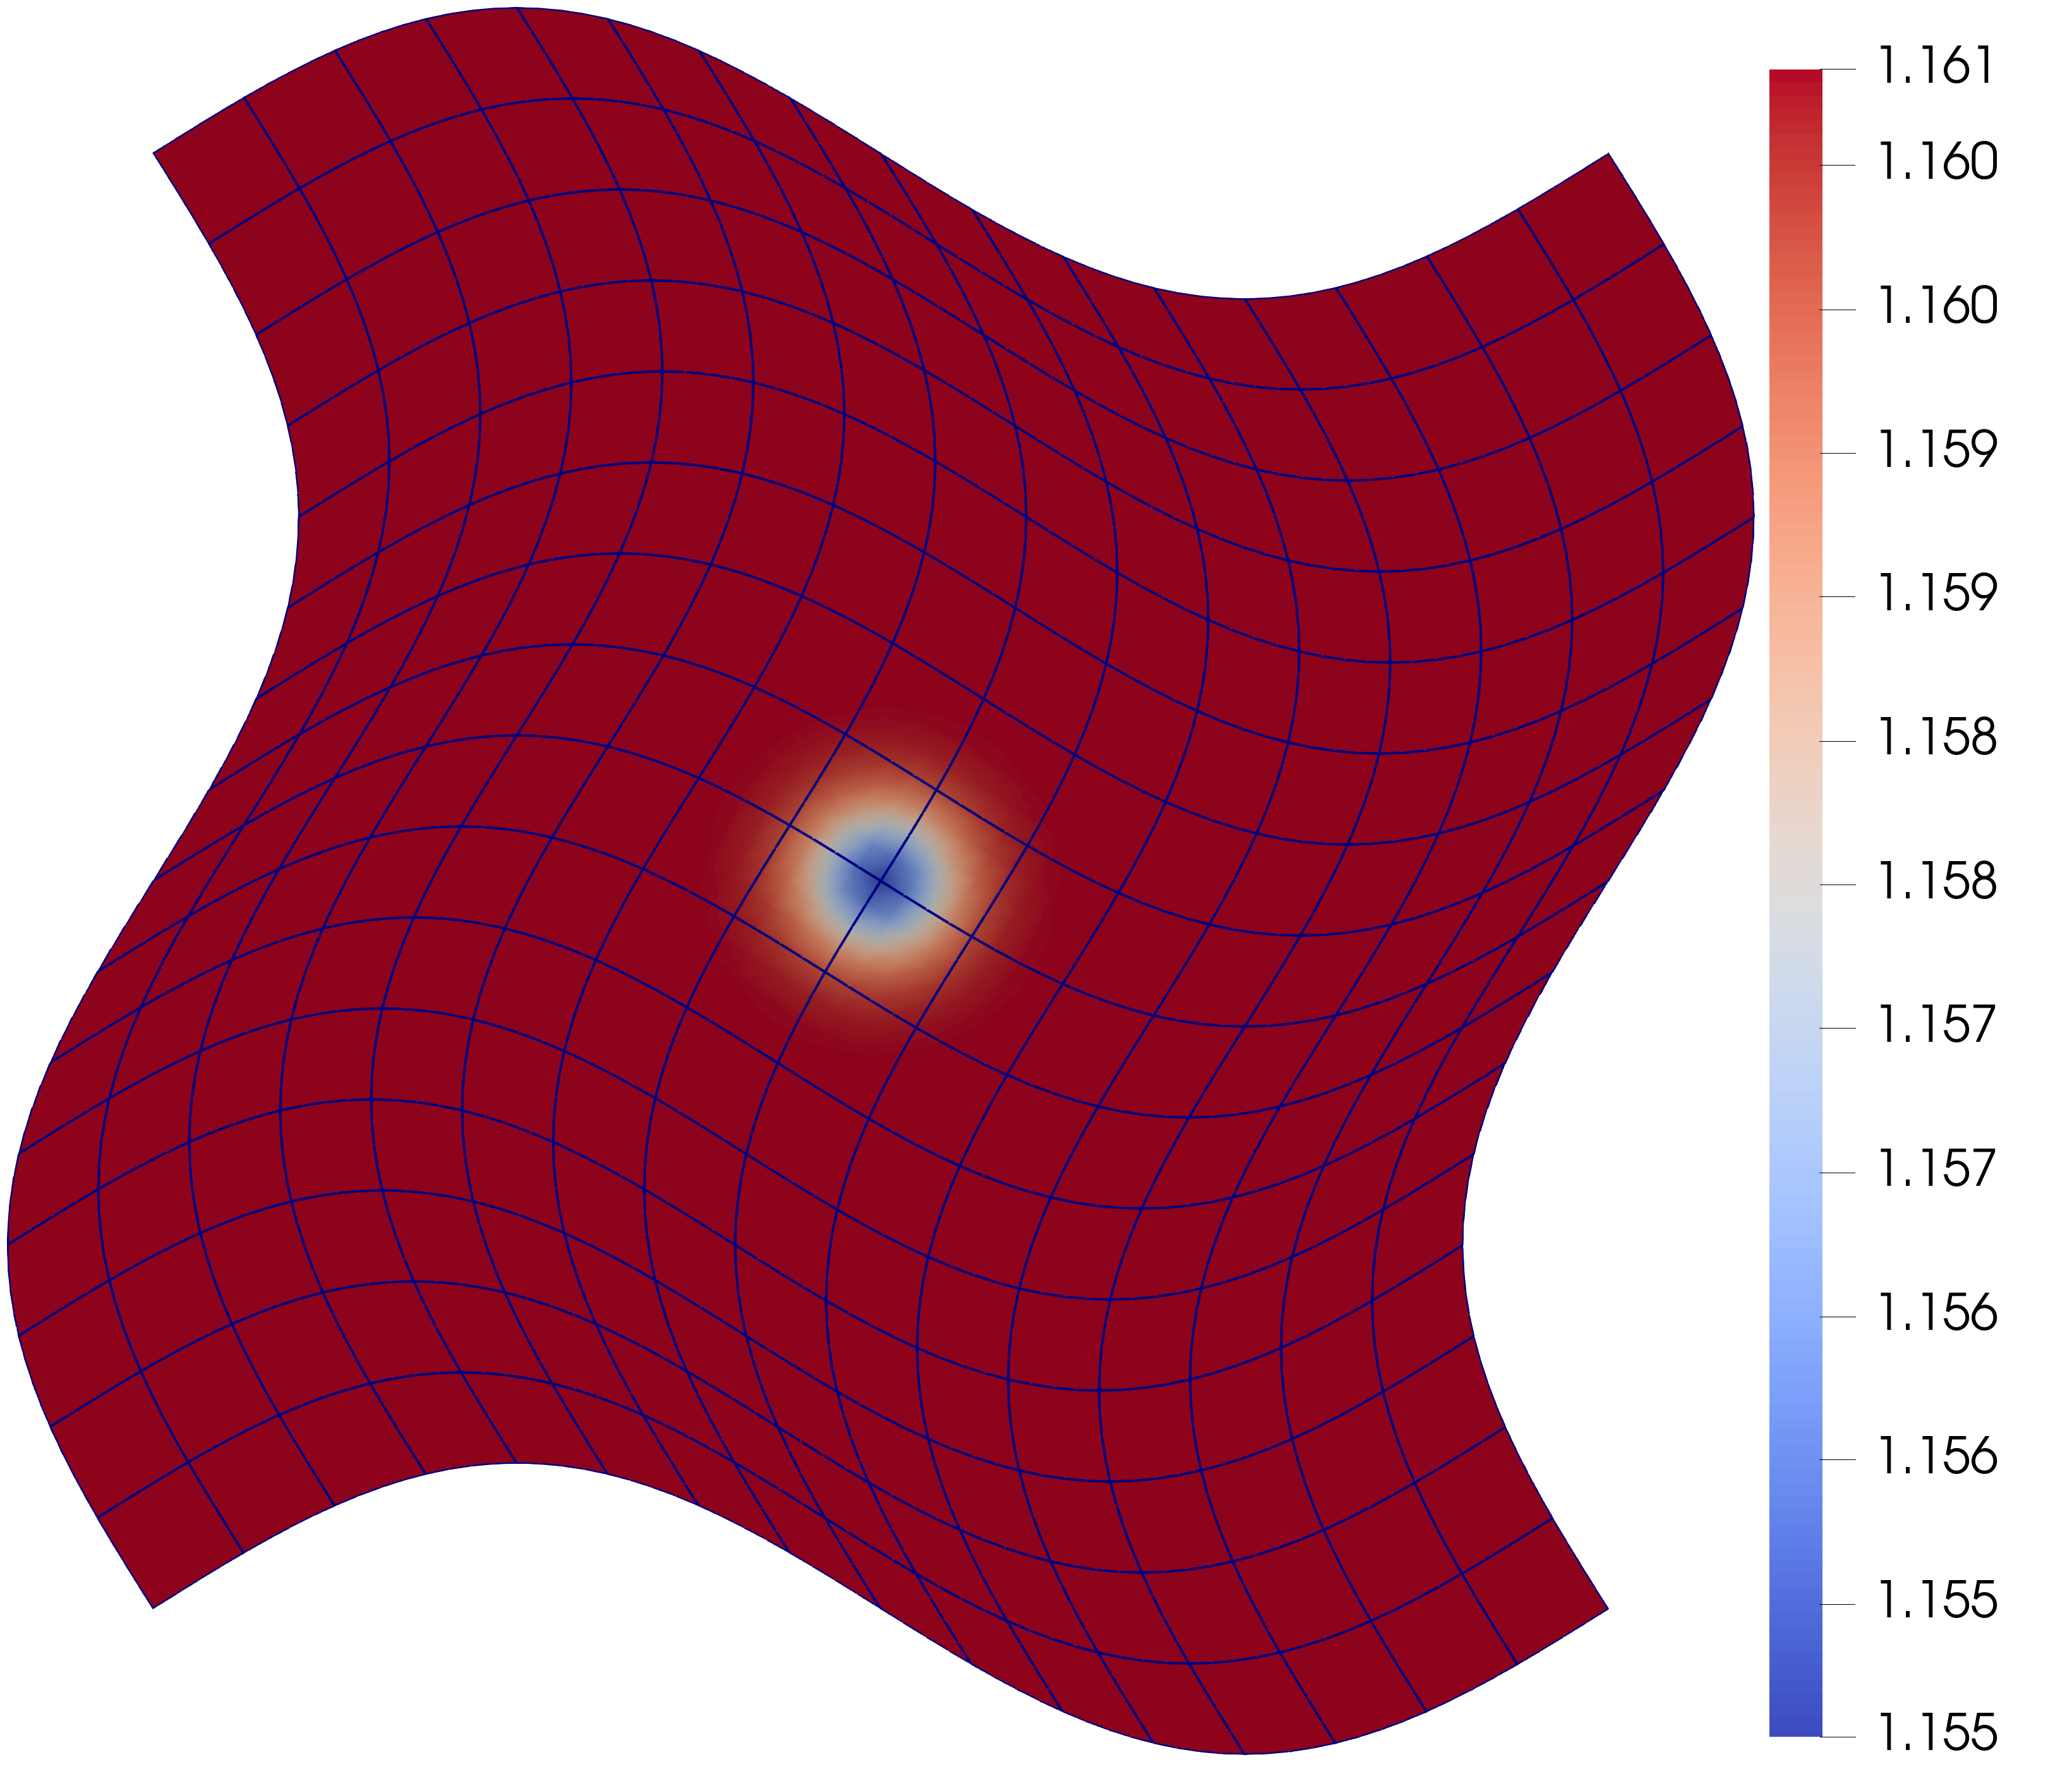
\includegraphics[width=0.9\linewidth]{attachments/isentropic_arpit.png}
        \caption*{(a)}
    \end{minipage}%
    \begin{minipage}{0.5\textwidth}
        \centering
        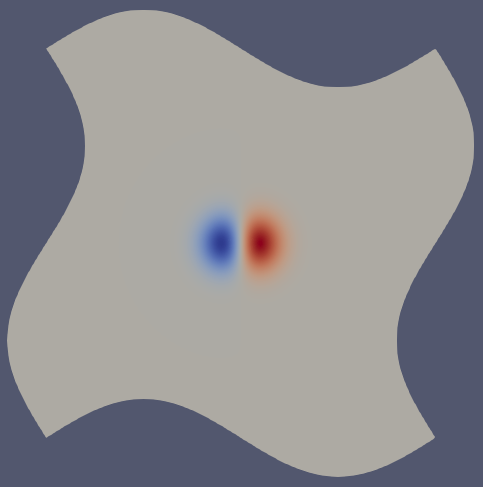
\includegraphics[width=0.9\linewidth]{attachments/solution_068877_vx.png}
        \caption*{(b)}
    \end{minipage}
    \caption{Isentropic vortex using polynomial degree $N = 4$, (a) density plot, (b) velocity in x direction}
\end{figure*}
\section{Scaling test} \label{st}
The numbers in speedup and efficiency that we got in results shows a promising hope for the problems of real world involving complex CFD simulations, big data etc., to be simulated using multi-node environment. These results can be improved further with better optimization techniques and utilising the features of modern hardware such as vector processors etc. 


\begin{center}
    \rule{3cm}{1pt}
\end{center}

\chapter{Conclusion} \label{c}
The results presented in chapter \ref{ai}, shows us that the real world problems that are data intensive and memory consuming, can be simulated with the help of parallel processing. They can be simulated with a good speedup and can utilize the hardware capabilities quiet effectively as shown by the results of efficiency. With harnessing the computing power and with larger pool of memory of many nodes connected with fast interconnects, we can simulate large problem in the fields of computational fluid dynamics, medical simulations, big data and many more.  

\vspace{10pt}
\hspace{-18pt}We also have proposed a alternative methodology for parallelization in chapter \ref{am}. The implementation has not been done yet for alternative methodology and that remains the work for future projects. 

\vspace{10pt}
\hspace{-18pt}The code following the methodology presented in chapter \ref{m} is available on Github but currently it is private. This code can be accessed on this \href{https://github.com/Arpit-Babbar/TrixiLW.jl/}{link} after the paper \cite{arpit} gets accepted for publication.

\chapter{Results} \label{ra}
The results (all results segregated at at a place)

% \chapter*{References}
\begin{thebibliography}{100}
\bibitem{notes_ncm}
Chandrashekar, P. (2019). {\em Numerical methods for hyperbolic system of conservation laws}. \href{https://math.tifrbng.res.in/~praveen/pub/ncm2019.pdf}{https://math.tifrbng.res.in/~praveen/pub/ncm2019.pdf}

\bibitem{rusanov}
V.V Rusanov (1962). {\em The calculation of the interaction of non-stationary shock waves and obstacles}. USSR Computational Mathematics and Mathematical Physics, 1(2), 304-320.

\bibitem{trojak}
W. TROJAK AND F. D. WITHERDEN, {\em A new family of weighted one-parameter flux reconstruction schemes, Computers \& Fluids}, 222 (2021), p. 104918.

\bibitem{hyunh}
H. T. HUYNH, {\em A Flux Reconstruction Approach to High-Order Schemes Including Discontinuous Galerkin Methods}, Miami, FL, June 2007, AIAA.

\bibitem{vincent}
P. VINCENT, F. WITHERDEN, B. VERMEIRE, J. S. PARK, AND A. IYER, {\em Towards Green Aviation with Python at Petascale, in SC16: International Conference for High Performance Computing, Networking, Storage and Analysis}, Salt Lake City, UT, Nov. 2016, IEEE, pp. 1-11.

\bibitem{trixi}
Schlottke-Lakemper, M., Gassner, G. J., Ranocha, H., Winters, A. R., \& Chan, J. (2024). {\em Trixi.jl (v0.8.3)}. Zenodo. \href{https://doi.org/10.5281/zenodo.12683615}{https://doi.org/10.5281/zenodo.12683615}

\bibitem{rma}
Hoefler, T., Balaji, P., Gropp, W., \& Thakur, R. (2016, November). \textit{Advanced MPI Programming} [Tutorial] \href{https://web.cels.anl.gov/ thakur/sc16-mpi-tutorial/slides.pdf}{https://web.cels.anl.gov/ thakur/sc16-mpi-tutorial/slides.pdf}

\bibitem{rmabook}
Hoefler, T., Gropp, W., Thakur, R., \& Lusk, E. (2014). \textit{Using advanced MPI: Modern features of the message-Passing-Interface.} MIT Press.

\bibitem{arpit}
Babbar, A., \& Chandrashekar, P. (2024). \textit{Lax-Wendroff Flux Reconstruction on adaptive curvilinear meshes with error based time stepping for hyperbolic conservation laws.} arXiv e-prints, arXiv:2402.11926.

\end{thebibliography}

\chapter*{Declaration}
\begin{figure*}[ht]
    \centering
    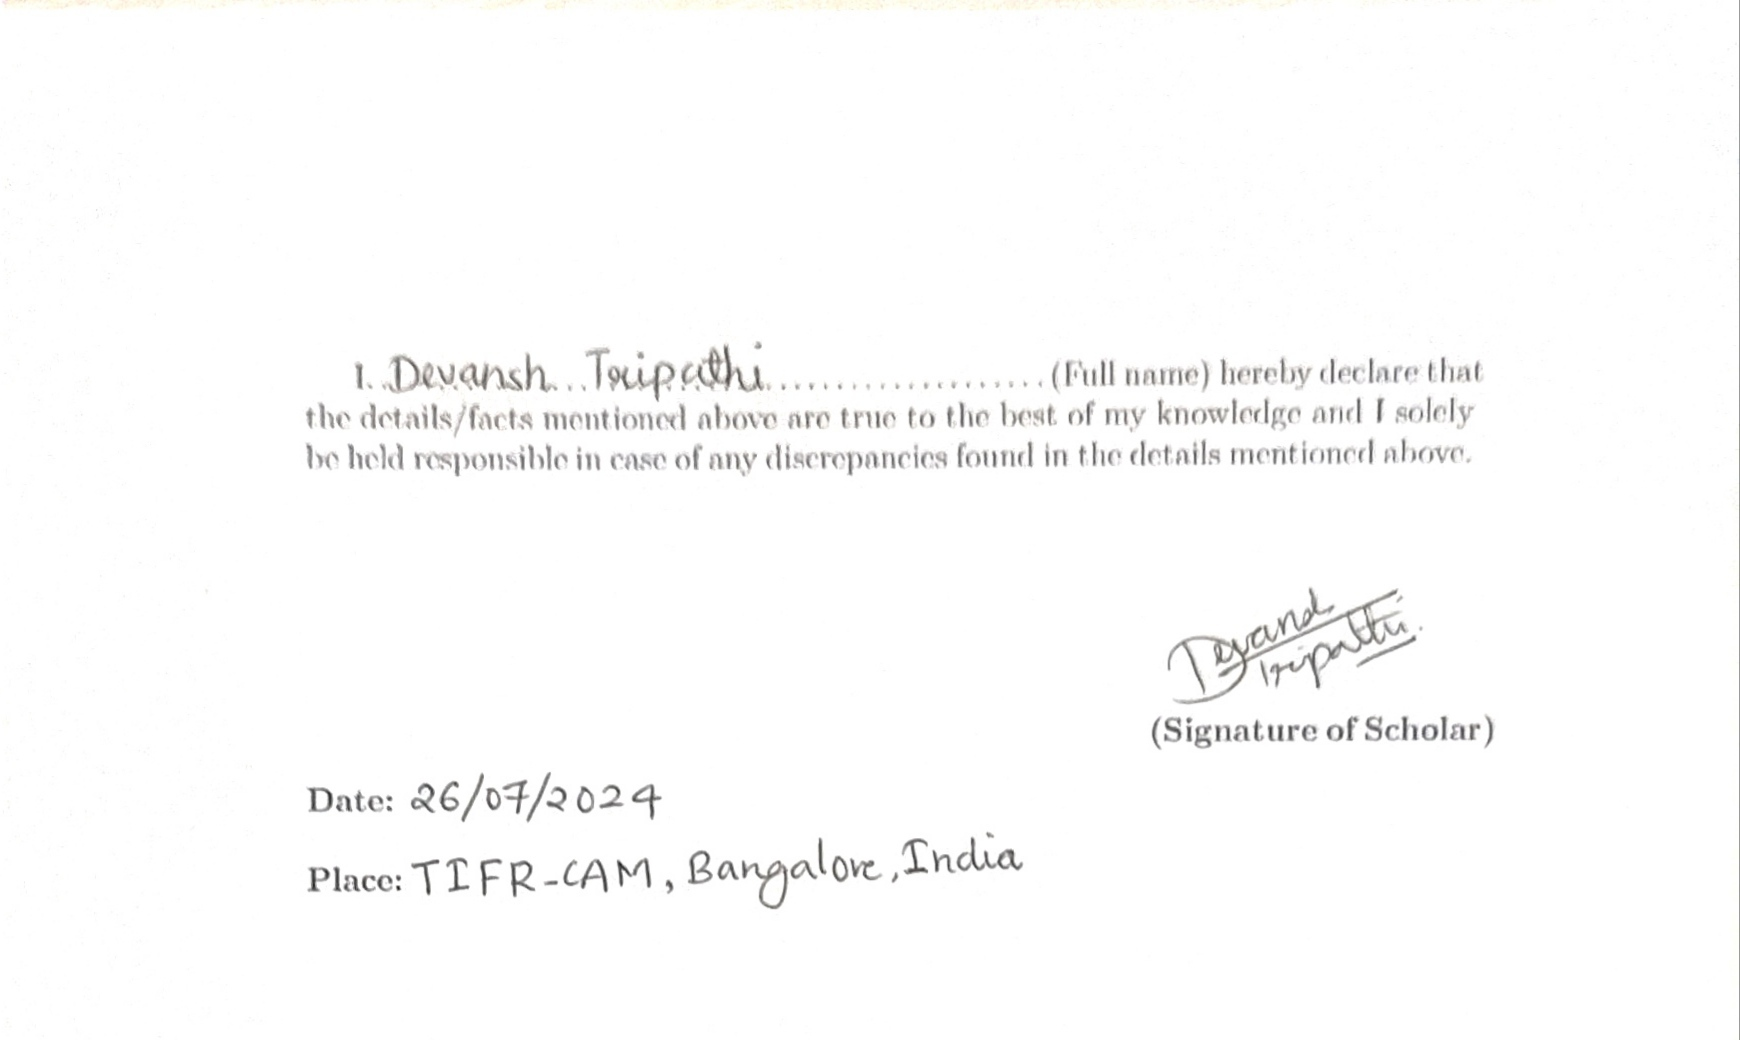
\includegraphics[width=0.95\linewidth]{attachments/declaration.jpg}
\end{figure*}

\end{document}